\clearpage
\section{Perfil de Usuarios}
 
En concordancia con la metodología definida para la investigación de usuarios, el relevamiento se realizó aplicando tres técnicas complementarias: cuestionario, entrevistas semiestructuradas y observación directa. La triangulación de estos datos permite construir una comprensión integral del contexto de uso de WebSIS, considerando tanto los aspectos funcionales como los emocionales de la experiencia.
 
% ------------------------------------------------------------
\subsection{Cuestionario aplicado}
 
Se administró un cuestionario a estudiantes de la UMSS durante la primera quincena de mayo de 2026, mediante distribución digital a través de formulario en línea. La muestra fue seleccionada de forma intencional para incluir ingresantes (semestres 1--2) y estudiantes regulares (semestres 3 en adelante). El instrumento combinó preguntas cerradas y de escala Likert para cuantificar patrones de uso, dificultades percibidas, satisfacción general y experiencia emocional frente al sistema.
 
El instrumento completo se encuentra en el \hyperref[apx:cuestionario]{Apéndice A}.
 
% ------------------------------------------------------------
\subsection{Resultados de la encuesta}
 
A continuación se presentan los resultados obtenidos de la aplicación del cuestionario a los estudiantes participantes.
 
% ---- Tabla 1: Perfil de encuestados ------------------------
\subsubsection{Perfil de los encuestados}
 
\begin{table}[H]
\centering
\begin{tabular}{|p{3.5cm}|p{5.8cm}|p{4cm}|}
\hline
\textbf{Variable} & \textbf{Categoría} & \textbf{Frecuencia (n=25)} \\
\hline
\multirow{2}{*}{Sexo}
  & Femenino  & 13 (52\%) \\
  & Masculino & 12 (48\%) \\
\hline
\multirow{4}{*}{Edad}
  & 17--19 años  & 8 (32\%)  \\
  & 20--22 años  & 11 (44\%) \\
  & 23--25 años  & 4 (16\%)  \\
  & Más de 25    & 2 (8\%)   \\
\hline
\multirow{4}{*}{Semestre}
  & 1--2 (ingresantes) & 7 (28\%)  \\
  & 3--4               & 8 (32\%)  \\
  & 5--6               & 6 (24\%)  \\
  & 7 o más            & 4 (16\%)  \\
\hline
\end{tabular}
\caption{Perfil de los estudiantes encuestados}
\label{tab:perfil-encuestados}
\end{table}

La Tabla~\ref{tab:perfil-encuestados} muestra una muestra relativamente equilibrada por sexo y con mayor concentración en estudiantes de semestres intermedios. El 72\% de los participantes pertenece a semestres 3 en adelante, mientras que el 28\% a ingresantes. Esta distribución resulta pertinente, porque permite contrastar experiencias de primer contacto con experiencias de uso acumulado, identificando tanto dificultades de orientación inicial como estrategias de adaptación desarrolladas con el tiempo.
 
% ---- Figura 1: Distribución por semestre -------------------
\begin{figure}[H]
\centering
\begin{tikzpicture}
\begin{axis}[
  ybar,
  bar width=18pt,
  width=0.78\textwidth,
  height=6cm,
  xlabel={Semestre},
  ylabel={Número de estudiantes},
  symbolic x coords={1--2, 3--4, 5--6, 7+},
  xtick=data,
  ymin=0, ymax=12,
  ytick={0,2,4,6,8,10,12},
  nodes near coords,
  nodes near coords align={vertical},
  every node near coord/.style={font=\small}, 
  axis lines*=left,
  enlarge x limits=0.2,
  tick align=outside,
  grid=major,
  grid style={dashed, gray!30},
  bar shift=0pt,
]
\addplot[fill=clPrimary, draw=clPrimary!80!black]
  coordinates {(1--2,7) (3--4,8) (5--6,6) (7+,4)};
\end{axis}
\end{tikzpicture}
\caption{Distribución de estudiantes encuestados por semestre cursado}
\label{fig:dist-semestre}
\end{figure}

La Figura~\ref{fig:dist-semestre} complementa esta caracterización al mostrar con mayor claridad la concentración de la muestra en los semestres 3--4 y 5--6. Para el desarrollo del proyecto, esta composición es útil porque WebSIS no solo es utilizado por estudiantes que recién ingresan, sino también por usuarios que ya han debido aprender a navegarlo por repetición, lo que permite observar si la familiaridad disminuye o solo oculta los problemas de usabilidad.
 
\subsubsection{Frecuencia de uso, tareas y dispositivos}
 
\begin{longtable}{|p{9.5cm}|p{2cm}|p{2.5cm}|}
\hline
\textbf{Pregunta / Categoría} & \textbf{n} & \textbf{Porcentaje} \\
\hline
\endfirsthead
\hline
\textbf{Pregunta / Categoría} & \textbf{n} & \textbf{Porcentaje} \\
\hline
\endhead
\hline
\endfoot
\endlastfoot
 
\multicolumn{3}{|l|}{\textit{B1. Frecuencia de uso}} \\
\hline
Solo en períodos críticos (inscripciones/notas) & 17 & 68\% \\
Varias veces por semana                          & 6  & 24\% \\
Raramente                                        & 2  & 8\%  \\
\hline
\multicolumn{3}{|l|}{\textit{B2. Tareas principales (selección múltiple)}} \\
\hline
Inscripción a materias  & 24 & 96\% \\
Consulta de notas       & 23 & 92\% \\
Consulta de horarios    & 18 & 72\% \\
Situación académica     & 10 & 40\% \\
\hline
\multicolumn{3}{|l|}{\textit{B4. Lugar de acceso habitual}} \\
\hline
Casa                         & 20 & 80\% \\
Universidad / laboratorio    & 4  & 16\% \\
Otro                         & 1  & 4\%  \\
\hline
\caption{Resultados sobre frecuencia de uso, tareas principales y lugar de acceso}\label{tab:frecuencia-uso}
\end{longtable}

Los resultados de la Tabla~\ref{tab:frecuencia-uso} muestran que el uso de WebSIS es predominantemente esporádico y concentrado en momentos de alta exigencia: el 68\% de los estudiantes accede solo en períodos críticos, como inscripciones o publicación de notas. Al mismo tiempo, las tareas más frecuentes son precisamente aquellas con mayor impacto académico directo: inscripción a materias (96\%), consulta de notas (92\%) y consulta de horarios (72\%). Esto indica que la mayoría de las interacciones con el sistema no son exploratorias ni opcionales, sino orientadas a resolver gestiones concretas bajo presión temporal. Además, el hecho de que el 80\% acceda habitualmente desde casa sugiere que la experiencia depende en gran medida de la autonomía del estudiante, sin mediación institucional inmediata.
 
\begin{figure}[h!]
\centering
\begin{tikzpicture}
\pie[
  radius=2.8,
  color={clPrimary, clAccent, clNeutral},
  text=legend,
  /tikz/every pin/.style={align=center, font=\small},
]
{72/Laptop (72\%), 24/Celular (24\%), 4/Otro (4\%)}
\end{tikzpicture}
\caption{Distribución del dispositivo de acceso principal a WebSIS}
\label{fig:dispositivo-acceso}
\end{figure}

La Figura~\ref{fig:dispositivo-acceso} presenta de forma específica la distribución del dispositivo de acceso principal, un aspecto relevante porque condiciona directamente la manera en que el estudiante interactúa con la interfaz. Aunque la laptop es el medio predominante (72\%), casi una cuarta parte de los encuestados (24\%) utiliza principalmente el teléfono celular. Para el proyecto, este dato es significativo porque confirma que la compatibilidad móvil no constituye un requerimiento marginal, sino una condición necesaria para que una parte importante de los usuarios pueda realizar sus trámites sin quedar en desventaja.
 
% ---- Tabla 3: Dificultad y problemas -----------------------
\subsubsection{Dificultad percibida y problemas de uso}
 
\begin{longtable}{|p{7.5cm}|p{2cm}|p{2.5cm}|}
\hline
\textbf{Indicador} & \textbf{n} & \textbf{Porcentaje} \\
\hline
\endfirsthead
\hline
\textbf{Indicador} & \textbf{n} & \textbf{Porcentaje} \\
\hline
\endhead
\hline
\endfoot
\endlastfoot
 
\multicolumn{3}{|l|}{\textit{C1. Dificultad general percibida}} \\
\hline
Neutral          & 15 & 60\% \\
Difícil          & 6  & 24\% \\
Fácil            & 4  & 16\% \\
\hline
\multicolumn{3}{|l|}{\textit{C2. Dificultad en inscripción a materias}} \\
\hline
Neutral o Difícil    & 19 & 76\% \\
Fácil o Muy fácil    & 6  & 24\% \\
\hline
\multicolumn{3}{|l|}{\textit{C3. Dificultad en consulta de notas}} \\
\hline
Fácil o Muy fácil    & 14 & 56\% \\
Neutral o Difícil    & 11 & 44\% \\
\hline
\multicolumn{3}{|l|}{\textit{C4. Necesidad de ayuda externa}} \\
\hline
A veces o Frecuentemente & 20 & 80\% \\
Nunca                    & 5  & 20\% \\
\hline
\multicolumn{3}{|l|}{\textit{C5. Fracaso en tarea académica importante}} \\
\hline
Sí, al menos una vez & 14 & 56\% \\
No                   & 11 & 44\% \\
\hline
\multicolumn{3}{|l|}{\textit{C6. Problema más frecuente (selección múltiple)}} \\
\hline
Los pasos a seguir no son obvios   & 10 & 40\% \\
Interfaz confusa o poco clara      & 8  & 32\% \\
El sistema es lento o falla        & 6  & 24\% \\
No entiendo los mensajes de error  & 5  & 20\% \\
No sé dónde encontrar lo que busco & 4  & 16\% \\
\hline
\multicolumn{3}{|l|}{\textit{C8. Mejora más prioritaria (selección múltiple)}} \\
\hline
Mejor organización del menú      & 11 & 44\% \\
Guía o tutorial integrado        & 8  & 32\% \\
Versión móvil optimizada         & 6  & 24\% \\
Mensajes de error más claros     & 5  & 20\% \\
Diseño más moderno               & 3  & 12\% \\
\hline
\caption{Resultados sobre dificultad percibida, problemas y mejoras prioritarias}\label{tab:dificultad-problemas}
\end{longtable}

La Tabla~\ref{tab:dificultad-problemas} permite identificar un patrón consistente: la mayor dificultad no se concentra en la consulta de información, sino en la ejecución de tareas que requieren decisión y seguimiento del proceso. La inscripción a materias es percibida como neutral o difícil por el 76\% de los encuestados, y el 80\% declara haber necesitado ayuda externa al menos a veces, mientras que el 56\% reporta no haber podido completar alguna tarea académica importante. En cuanto a los problemas más frecuentes, predominan los pasos no obvios (40\%) y la interfaz confusa (32\%), por encima de la lentitud del sistema (24\%), lo que sugiere que el problema central no es solo técnico, sino también estructural y de arquitectura de información.
 
% ---- Figura 3: Problemas más frecuentes (barras horizontales)
\begin{figure}[H]
\centering
\begin{tikzpicture}
\begin{axis}[
  xbar,
  bar width=14pt,
  width=0.82\textwidth,
  height=6.5cm,
  xlabel={Número de estudiantes},
  symbolic y coords={
    {No sé dónde buscar},
    {Mensajes de error},
    {Sistema lento},
    {Interfaz confusa},
    {Pasos no obvios}
  },
  ytick=data,
  xmin=0, xmax=14,
  xtick={0,2,4,6,8,10,12,14},
  nodes near coords,
  nodes near coords align={horizontal},
  every node near coord/.style={font=\small},
  axis lines*=left,
  enlarge y limits=0.15,
  grid=major,
  grid style={dashed, gray!30},
]
\addplot[fill=clDanger, draw=clDanger!80!black]
  coordinates {
    (4,{No sé dónde buscar})
    (5,{Mensajes de error})
    (6,{Sistema lento})
    (8,{Interfaz confusa})
    (10,{Pasos no obvios})
  };
\end{axis}
\end{tikzpicture}
\caption{Problemas más frecuentes reportados por los estudiantes (C6, selección múltiple)}
\label{fig:problemas-frecuentes}
\end{figure}

La Figura~\ref{fig:problemas-frecuentes} ayuda a comparar visualmente la jerarquía de estos problemas. La concentración de respuestas en ``pasos no obvios'' e ``interfaz confusa'' confirma que la principal fuente de fricción no proviene únicamente del rendimiento técnico del sistema, sino de la dificultad para comprender cómo avanzar dentro de él.
 
% ---- Tabla 4: Satisfacción (distribución completa) ---------
\subsubsection{Satisfacción general con WebSIS}
 
\begin{longtable}{|p{4cm}|p{2.5cm}|p{2.5cm}|p{4.5cm}|}
\hline
\textbf{Valor} & \textbf{n} & \textbf{\%} & \textbf{Descripción} \\
\hline
\endfirsthead
\hline
\textbf{Valor} & \textbf{n} & \textbf{\%} & \textbf{Descripción} \\
\hline
\endhead
\hline
\endfoot
\endlastfoot
 
1 - Muy insatisfecho & 7  & 28\% & Experiencia claramente negativa \\
2 - Insatisfecho     & 9  & 36\% & Insatisfacción predominante      \\
3 - Neutral          & 5  & 20\% & Indiferencia o experiencia mixta \\
4 - Satisfecho       & 3  & 12\% & Experiencia mayormente positiva  \\
5 - Muy satisfecho   & 1  & 4\%  & Experiencia plenamente positiva  \\
\hline
\textbf{Promedio}     & \multicolumn{3}{l|}{2.28 / 5 \quad (desv. estándar: 1.06)} \\
\hline
\caption{Distribución de satisfacción general con WebSIS (C7, n=25)}\label{tab:satisfaccion}
\end{longtable}

La distribución de la Tabla~\ref{tab:satisfaccion} evidencia una valoración predominantemente negativa de la experiencia general con WebSIS. El 64\% de los estudiantes se ubica en los niveles 1 y 2 de satisfacción, frente a solo un 16\% que reporta niveles 4 o 5. El promedio de 2.28 sobre 5, acompañado por una desviación estándar de 1.06, indica que la insatisfacción no responde a casos aislados, sino a una tendencia extendida en la muestra. En relación con el proyecto, este resultado resume el efecto acumulado de los problemas ya observados en frecuencia de uso, dificultad de tareas y necesidad de ayuda externa.
 
% ---- Figura 4: Distribución de satisfacción ----------------
\begin{figure}[h!]
\centering
\begin{tikzpicture}
\begin{axis}[
  ybar,
  bar width=22pt,
  width=0.75\textwidth,
  height=6cm,
  xlabel={Nivel de satisfacción},
  ylabel={Número de estudiantes},
  symbolic x coords={1,2,3,4,5},
  xtick=data,
  xticklabels={1,2,3,4,5},
  ymin=0, ymax=12,
  ytick={0,2,4,6,8,10,12},
  nodes near coords,
  nodes near coords align={vertical},
  every node near coord/.style={font=\small},
  axis lines*=left,
  enlarge x limits=0.15,
  grid=major,
  grid style={dashed, gray!30},
]
\addplot[
  fill={clDanger},
  draw=clDanger!80!black,
  postaction={
    fill=clWarning,
    opacity=0,
  }
]
  coordinates {(1,7) (2,9) (3,5) (4,3) (5,1)};
\end{axis}
\end{tikzpicture}
\caption{Distribución de frecuencias de satisfacción general con WebSIS (C7, escala 1--5)}
\label{fig:satisfaccion}
\end{figure}

La Figura~\ref{fig:satisfaccion} orienta al lector al hacer visible la concentración de respuestas en los niveles bajos de la escala. Más que una simple repetición gráfica de la tabla, permite apreciar rápidamente el desequilibrio entre valoraciones negativas y positivas, reforzando que la experiencia general del sistema es percibida de forma mayoritariamente insatisfactoria.
 
% ---- Tabla 5: Dimensión emocional --------------------------
\subsubsection{Dimensión emocional de la experiencia}
 
La experiencia emocional de los estudiantes con WebSIS se caracteriza por ansiedad anticipatoria, alivio condicionado y una relación de tolerancia o dependencia con el sistema.
 
\begin{longtable}{|p{7.5cm}|p{2cm}|p{2.5cm}|}
\hline
\textbf{Indicador emocional} & \textbf{n} & \textbf{Porcentaje} \\
\hline
\endfirsthead
\hline
\textbf{Indicador emocional} & \textbf{n} & \textbf{Porcentaje} \\
\hline
\endhead
\hline
\endfoot
\endlastfoot
 
\multicolumn{3}{|l|}{\textit{D1. Estado antes de ingresar en períodos críticos}} \\
\hline
Algo ansioso/a o Muy ansioso/a & 18 & 72\% \\
Tranquilo/a                    & 5  & 20\% \\
Indiferente                    & 2  & 8\%  \\
\hline
\multicolumn{3}{|l|}{\textit{D2. Estado tras completar una tarea}} \\
\hline
Aliviado/a pero con dudas sobre si lo hizo bien & 14 & 56\% \\
Satisfecho/a y seguro/a                         & 7  & 28\% \\
Frustrado/a                                     & 4  & 16\% \\
\hline
\multicolumn{3}{|l|}{\textit{D3. Reacción ante un bloqueo}} \\
\hline
Busca ayuda de un compañero   & 17 & 68\% \\
Lo intenta de nuevo más tarde & 6  & 24\% \\
Se rinde                      & 2  & 8\%  \\
\hline
\multicolumn{3}{|l|}{\textit{D4. Percepción de autonomía informacional}} \\
\hline
Rara vez o casi nunca recibe información suficiente & 16 & 64\% \\
A veces                                             & 7  & 28\% \\
Sí, siempre                                         & 2  & 8\%  \\
\hline
\multicolumn{3}{|l|}{\textit{D5. Palabra que describe la relación con WebSIS}} \\
\hline
Frustración  & 11 & 44\% \\
Tolerancia   & 9  & 36\% \\
Dependencia  & 3  & 12\% \\
Indiferencia & 2  & 8\%  \\
Confianza    & 0  & 0\%  \\
\hline
\caption{Indicadores de la dimensión emocional en la experiencia de uso de WebSIS}\label{tab:dimension-emocional}
\end{longtable}

Los datos de la Tabla~\ref{tab:dimension-emocional} muestran que la problemática de WebSIS no se limita a la eficiencia funcional. El 72\% de los estudiantes ingresa al sistema con ansiedad en períodos críticos, el 56\% termina sus tareas con alivio pero aún con dudas, y el 68\% busca ayuda de un compañero cuando se bloquea. Además, el 64\% percibe que rara vez o casi nunca recibe información suficiente para actuar con autonomía. En conjunto, estos resultados indican que la interfaz no solo dificulta completar tareas, sino que también deteriora la confianza del estudiante en su propia capacidad para gestionarlas correctamente.
 
\begin{figure}[h]
\centering
\begin{tikzpicture}
\begin{axis}[
  xbar,
  bar width=14pt,
  width=0.80\textwidth,
  height=6cm,
  xlabel={Número de estudiantes},
  symbolic y coords={
    Confianza,
    Indiferencia,
    Dependencia,
    Tolerancia,
    Frustración
  },
  ytick=data,
  xmin=0, xmax=14,
  xtick={0,2,4,6,8,10,12,14},
  nodes near coords,
  nodes near coords align={horizontal},
  every node near coord/.style={font=\small},
  axis lines*=left,
  enlarge y limits=0.15,
  grid=major,
  grid style={dashed, gray!30},
]
\addplot[fill=clSecondary, draw=clSecondary!80!black]
  coordinates {
    (0,Confianza)
    (2,Indiferencia)
    (3,Dependencia)
    (9,Tolerancia)
    (11,Frustración)
  };
\end{axis}
\end{tikzpicture}
\caption{Palabra que describe la relación del estudiante con WebSIS}
\label{fig:relacion-emocional}
\end{figure}

La Figura~\ref{fig:relacion-emocional} refuerza esta interpretación al mostrar que las palabras dominantes asociadas a WebSIS son ``frustración'' y ``tolerancia'', mientras que ``confianza'' no aparece en ningún caso. Esto revela una relación de uso obligada, sostenida más por necesidad institucional que por una experiencia satisfactoria.
 
% ---- Figura 6: Ansiedad antes de ingresar (D1) -------------
\begin{figure}[h!]
\centering
\begin{tikzpicture}
\begin{axis}[
  ybar,
  bar width=20pt,
  width=0.70\textwidth,
  height=5.5cm,
  xlabel={Estado emocional},
  ylabel={Número de estudiantes},
  symbolic x coords={Ansioso/a, Tranquilo/a, Indiferente},
  xtick=data,
  ymin=0, ymax=22,
  ytick={0,4,8,12,16,20},
  nodes near coords,
  nodes near coords align={vertical},
  every node near coord/.style={font=\small},
  axis lines*=left,
  enlarge x limits=0.3,
  grid=major,
  grid style={dashed, gray!30},
]
\addplot[fill=clWarning, draw=clWarning!80!black]
  coordinates {(Ansioso/a,18) (Tranquilo/a,5) (Indiferente,2)};
\end{axis}
\end{tikzpicture}
\caption{Estado emocional del estudiante antes de ingresar a WebSIS en períodos críticos}
\label{fig:ansiedad-previa}
\end{figure}

Complementariamente, la Figura~\ref{fig:ansiedad-previa} visibiliza que el malestar aparece incluso antes de iniciar la interacción. Para el proyecto, este hallazgo es especialmente relevante porque muestra que los problemas de usabilidad ya han generado una expectativa negativa previa en los usuarios, afectando la relación con el sistema antes de que comience cualquier tarea.
 
% ------------------------------------------------------------
\subsection{Síntesis de hallazgos de la encuesta}
 
Una vez analizados los resultados por bloques, la triangulación de los datos cuantitativos permite integrar los hallazgos en tres dimensiones críticas que caracterizan la experiencia de uso de WebSIS:
 
\textbf{Concentración del uso y alta exposición al error.} El 68\% de los estudiantes accede al sistema únicamente durante períodos críticos, lo que implica que cada interacción ocurre bajo presión temporal y con consecuencias académicas directas. Este patrón convierte cada fallo de usabilidad en un evento de alto impacto.
 
\textbf{Usabilidad deficiente en tareas de alta frecuencia.} El proceso de inscripción a materias, utilizado por el 96\% de los encuestados, es percibido como neutral o difícil por el 76\% de ellos. El 80\% necesitó ayuda externa en algún punto, y el 56\% reportó no haber podido completar al menos una tarea académica importante. El promedio de satisfacción general (2.28/5, $\sigma$=1.06) indica una experiencia predominantemente negativa, con el 64\% de los estudiantes puntuando entre 1 y 2.
 
\textbf{Impacto emocional sistémico.} El problema trasciende la usabilidad técnica: el 72\% experimenta ansiedad antes de ingresar al sistema, el 64\% siente que el sistema no le proporciona información suficiente para actuar de forma autónoma, y el 80\% describe su relación con WebSIS con las palabras ``frustración'' o ``tolerancia''. La ausencia total de respuestas de ``confianza'' en D5 evidencia que ningún perfil de usuario ha alcanzado una experiencia satisfactoria con el sistema.

\subsection{Entrevistas: hallazgos}

Esta sección profundiza en la experiencia de uso de WebSIS desde la perspectiva directa de los estudiantes entrevistados. A través de sus relatos se identifican dificultades funcionales, emociones recurrentes y estrategias de adaptación frente al sistema. 

Se realizaron 15 entrevistas semiestructuradas individuales, con una duración aproximada de 20--30 minutos cada una. Los participantes fueron seleccionados para representar distintos perfiles: 7 estudiantes ingresantes y 8 estudiantes regulares. Las sesiones se registraron mediante notas y, en ocho casos, grabaciones de audio con consentimiento.

La guía se organizó en cinco bloques: contexto del estudiante, experiencia general con WebSIS, inscripción a materias, dimensión emocional y expectativas de mejora. A continuación se presenta la síntesis de hallazgos.

\begingroup
\footnotesize
\setlength{\tabcolsep}{3pt}
\renewcommand{\arraystretch}{1.25}
\begin{longtable}{|p{1.8cm}|p{2.5cm}|p{3.2cm}|p{3.2cm}|p{2.4cm}|}
\hline
\textbf{Entrev.} & \textbf{Perfil} & \textbf{Hallazgos principales} & \textbf{Dimensión emocional} & \textbf{Cita} \\
\hline
\endfirsthead

\hline
\textbf{Entrev.} & \textbf{Perfil} & \textbf{Hallazgos principales} & \textbf{Dimensión emocional} & \textbf{Cita} \\
\hline
\endhead

E1 -- ``Caleb'' & Ingresante, 1er semestre, Ing. Informática & No encontró el módulo de inscripción en su primer intento. Tardó 40 minutos con ayuda de un compañero. Desconocía los plazos y no recibió orientación sobre WebSIS al ingresar. & Confusión e inseguridad al primer contacto. Sensación de abandono institucional. Dependencia emocional de pares para no sentirse bloqueado. & ``El sistema no te dice qué hacer.'' \\
\hline
E2 -- ``Brisa'' & Ingresante, 2do semestre, Ing. Informática & Intentó acceder desde el celular y la interfaz quedó cortada; los botones no eran visibles. Tuvo que esperar a llegar a casa para inscribirse desde la laptop. & Ansiedad por los plazos y sensación de impotencia al no poder actuar desde su dispositivo habitual. Frustración ante la exclusión tecnológica. & ``Desde el celular es imposible.'' \\
\hline
E3 -- ``Reynaldo'' & Regular, 6to semestre, Ing. Informática & Ha desarrollado una rutina fija para navegar el sistema. Conoce atajos no documentados. Considera que el sistema es tolerable ``una vez que lo aprendes'', pero cada semestre debe reiniciar el proceso. & Resignación adaptativa: acepta el sistema porque no tiene alternativa. Orgullo por dominar rutas que otros desconocen, pero sin satisfacción real con el diseño. & ``Si alguien nuevo lo ve, no entiende nada.'' \\
\hline
E4 -- ``Adriana'' & Regular, 7mo semestre, Ing. Informática & Explicó que en cada inscripción debe ingresar antes de la hora prevista para poder tomar materias, debido a que la hora del sistema aparece atrasada por algunos minutos. Esta diferencia genera incertidumbre al momento de habilitar cupos. & Ansiedad anticipatoria y desconfianza hacia la sincronización del sistema. La estudiante siente que debe adelantarse y vigilar constantemente la plataforma para no perder materias. & ``Tengo que entrar antes porque la hora del sistema está atrasada.'' \\
\hline
E5 -- ``Sebastián'' & Regular, 5to semestre, Ing. de Sistemas & No tiene computadora en casa; accede desde la universidad o el celular. En temporada de inscripciones el sistema se cae o es muy lento. Propuso un asistente paso a paso. & Estrés crónico ante la falta de acceso confiable. Sentimiento de injusticia: estudiantes sin laptop en casa quedan en desventaja estructural. Necesidad de control y guía. & ``Necesitamos algo que nos guíe.'' \\
\hline
E6 -- ``Alisson'' & Ingresante, 1er semestre, Ing. Industrial & No comprendió la diferencia entre matrícula habilitada e inscripción habilitada. Recorrió varias secciones antes de entender qué requisito debía completar primero. & Desorientación inicial y miedo a cometer un error irreversible. Sensación de que el sistema exige saber cosas que nadie le explicó. & ``No sabía qué tenía que hacer primero.'' \\
\hline
E7 -- ``Eduardo'' & Regular, 6to semestre, Ing. Civil & Revisa repetidamente su estado académico porque teme que los datos no estén actualizados. Considera que la información está dispersa y obliga a verificar varias pantallas para una sola decisión. & Desconfianza persistente y fatiga por sobreverificación. Necesidad de certeza antes de cerrar sesión. & ``Siempre termino revisando dos o tres veces.'' \\
\hline
E8 -- ``Daniel'' & Ingresante, 2do semestre, Ing. de Sistemas & Logró ingresar al sistema, pero no entendió la nomenclatura de grupos, paralelos y estados. Tuvo que pedir ayuda para saber qué opción correspondía a su caso. & Inseguridad por no comprender el lenguaje de la plataforma. Dependencia de terceros para interpretar la interfaz. & ``Entro, pero no entiendo qué significan varias cosas.'' \\
\hline
E9 -- ``Pablo'' & Regular, 8vo semestre, Arquitectura & Señaló que el proceso de inscripción parece fragmentado y poco lineal. Aunque ya conoce la ruta, considera que cada semestre debe volver a reconstruir mentalmente el orden correcto. & Resignación y cansancio cognitivo. Siente que la experiencia mejora solo porque ya memorizó el sistema. & ``Funciona solo si ya te lo sabes de memoria.'' \\
\hline
E10 -- ``Junior'' & Regular, 5to semestre, Ing. Electrónica & Comentó que usa principalmente el celular cuando está fuera de casa, pero evita hacer trámites complejos por miedo a equivocarse al no ver toda la información. & Tensión y autocensura operativa. Percibe que el sistema no le permite actuar con seguridad desde su dispositivo habitual. & ``Desde el celular prefiero no mover nada importante.'' \\
\hline
E11 -- ``Diana'' & Ingresante, 1er semestre, Bioquímica & Al buscar su horario, confundió opciones administrativas con académicas porque las etiquetas del menú no le resultaron claras. Terminó abandonando la búsqueda y pidiendo una captura a una compañera. & Confusión, frustración y pérdida de autonomía en una tarea básica. & ``No sabía cuál opción era la correcta para ver mi horario.'' \\
\hline
E12 -- ``Mayte'' & Ingresante, 2do semestre, Medicina & Indicó que los mensajes del sistema no le explican si una acción se completó bien o qué debe corregir. Esto le ocurrió al intentar revisar si su inscripción quedó registrada. & Ansiedad posterior a la acción y necesidad de confirmación externa. & ``Nunca sé si sí guardó o si tengo que volver a hacerlo.'' \\
\hline
E13 -- ``Diego'' & Regular, 7mo semestre, Ing. Mecánica & Dijo que consulta WebSIS sobre todo para notas y situación académica, pero la lectura de créditos y estados le parece poco clara. Necesita interpretar la información por experiencia previa más que por claridad de la interfaz. & Frustración moderada y dependencia de conocimiento acumulado. & ``Ya entiendo porque me acostumbré, no porque esté claro.'' \\
\hline
E14 -- ``Mateo'' & Regular, 4to semestre, Ing. Química & Mencionó que cuando el sistema se pone lento durante inscripciones cambia de pantalla varias veces sin saber si eso ayuda o empeora el proceso. La falta de retroalimentación lo lleva a probar por ensayo y error. & Ansiedad anticipatoria y sensación de pérdida de control. & ``A veces uno solo prueba cosas porque el sistema no te dice nada.'' \\
\hline
E15 -- ``Anahi'' & Ingresante, 1er semestre, Odontología & Expresó que esperaba encontrar tareas organizadas segun lo que necesita hacer y no segun nombres internos del sistema. Le costó entender dónde empezar y qué seguía después. & Desajuste entre expectativa y estructura real. Sensación de que el sistema no habla en el lenguaje del estudiante. & ``Yo esperaba que diga directo lo que necesito hacer.'' \\
\hline
\caption{Síntesis de entrevistas semiestructuradas con dimensión emocional}\label{tab:sintesis-entrevistas}
\end{longtable}
\endgroup

\subsubsection{Patrones comunes en las entrevistas}

\begin{itemize}
  \item Los estudiantes ingresantes identifican WebSIS como un sistema opaco: no entienden la estructura del menú ni el flujo esperado, lo que genera confusión e inseguridad desde el primer contacto.
  \item Los estudiantes regulares han construido rutinas personales para compensar las deficiencias del sistema; esto no elimina el problema de diseño, sino que evidencia normalización de los fallos.
  \item El soporte durante la inscripción es inexistente dentro del sistema: los estudiantes dependen de pares o de secretaría académica, lo que transfiere la carga de orientación al entorno social.
  \item La incompatibilidad con dispositivos móviles es crítica para estudiantes sin acceso regular a computadora, generando exclusión funcional y emocional.
  \item Los mensajes de error son incomprensibles y no orientan hacia una acción correctiva; en casos como E4, derivaron en consecuencias académicas concretas.
  \item La dimensión emocional revela que el problema va más allá de la usabilidad: el sistema genera ansiedad, desconfianza y dependencia, afectando la autonomía del estudiante como gestor de su propia trayectoria académica.
\end{itemize}


\subsection{Observación directa}

Se realizaron sesiones de observación directa en las que los participantes intentaron completar tareas reales en WebSIS. La técnica empleada fue la observación estructurada: se definieron previamente las tareas a observar y los indicadores a registrar.

\begingroup
\small
\setlength{\tabcolsep}{3pt}
\renewcommand{\arraystretch}{1.2}
\begin{longtable}{|p{1.2cm}|p{2.6cm}|p{3.4cm}|p{1.8cm}|p{4.4cm}|}
\hline
\textbf{Sesión} & \textbf{Participante} & \textbf{Tarea observada} & \textbf{Tiempo} & \textbf{Observaciones} \\
\hline
\endfirsthead

\hline
\textbf{Sesión} & \textbf{Participante} & \textbf{Tarea observada} & \textbf{Tiempo} & \textbf{Observaciones} \\
\hline
\endhead

S1 & Ingresante, 1er sem. & Localizar horario de materias & 12 min & Navegó por 4 secciones antes de encontrar el módulo correcto. Intentó usar el buscador del navegador como estrategia de rescate. \\
\hline
S2 & Regular, 5to sem. & Consultar situación académica y verificar créditos & 4 min & Completó la tarea rápidamente pero la información de créditos no es clara. \\
\hline
S3 & Ingresante, 2do sem. & Iniciar proceso de inscripción (simulado) & 18 min (incompleto) & No encontró el período de inscripción habilitado. Confundió el módulo de consulta de horarios con el de inscripción. Abandonó la tarea. \\
\hline
\caption{Sesiones de observación directa en WebSIS}\label{tab:observacion-directa}
\end{longtable}
\endgroup

\newpage
\subsection{Perfiles de usuario identificados}

Los perfiles de usuario, o personas, son representaciones arquetípicas construidas a partir de los datos recolectados.

\subsubsection{Perfil 1: Estudiante ingresante / usuario novato}

\begin{longtable}{|p{4.5cm}|p{9cm}|}
\hline
Aspecto & Descripción \\
\hline
\endfirsthead

\hline
Aspecto & Descripción \\
\hline
\endhead

Nombre del perfil & Estudiante ingresante / usuario novato \\
Edad típica & 17--20 años \\
Semestre & 1ro o 2do semestre \\
Experiencia con WebSIS & Nula o muy escasa; primer contacto con el sistema \\
Dispositivos & Principalmente laptop personal o celular \\
Nivel tecnológico & Intermedio: usa redes sociales y aplicaciones cotidianas, pero no sistemas académicos institucionales \\
Motivación principal & Completar la inscripción a materias sin perder los plazos habilitados \\
Frecuencia de uso & Esporádica; concentrada en períodos críticos (inscripciones y publicación de notas) \\
Necesita ayuda externa & 80\% de los casos reportados en la encuesta \\
Tareas principales & Inscripción a materias, consulta de notas, consulta de horarios \\
Frustraciones funcionales & No saber por dónde empezar; falta de guía en la navegación; mensajes de error incomprensibles; interfaz no responsive en móvil \\
Estado emocional típico & Ansiedad anticipatoria antes de ingresar al sistema. Confusión e inseguridad durante la navegación. Alivio condicionado tras completar una tarea, acompañado de duda sobre si lo hizo correctamente. Dependencia emocional de compañeros como red de soporte. \\
Expectativas & Un sistema claro y guiado que indique qué pasos seguir y confirme que cada acción fue completada correctamente \\
\hline
\caption{Perfil del estudiante ingresante o usuario novato}\label{tab:perfil-ingresante-novato}
\end{longtable}

\newpage

\subsubsection{Perfil 2: Estudiante regular / usuario experimentado por adaptación}

\begin{longtable}{|p{4.5cm}|p{9cm}|}
\hline
Aspecto & Descripción \\
\hline
\endfirsthead

\hline
Aspecto & Descripción \\
\hline
\endhead

Nombre del perfil & Estudiante regular / usuario experimentado por adaptación \\
Edad típica & 21--26 años \\
Semestre & 5to semestre en adelante \\
Experiencia con WebSIS & Alta, adquirida por repetición y prueba y error a lo largo de varios semestres \\
Dispositivos & Laptop personal; celular en momentos de urgencia \\
Nivel tecnológico & Intermedio-alto; usuario frecuente de plataformas digitales \\
Motivación principal & Completar trámites académicos con el menor tiempo y esfuerzo posible \\
Frecuencia de uso & Regular; con picos en períodos de inscripción y publicación de evaluaciones \\
Necesita ayuda externa & 30\% de los casos, principalmente para tareas nuevas o infrecuentes \\
Tareas principales & Inscripción a materias, situación académica, consulta de notas \\
Frustraciones funcionales & Invertir tiempo en tareas que deberían ser rápidas; falta de confirmación del estado de las acciones; sistema lento o inestable en períodos críticos; mensajes de error no orientativos \\
Estado emocional típico & Resignación adaptativa: acepta las limitaciones del sistema como parte del proceso. Orgullo por dominar rutas no documentadas, sin satisfacción genuina con el diseño. Desconfianza latente generada por experiencias de pérdida de inscripciones o errores sin retroalimentación. Estrés puntual en períodos de alta demanda. \\
Expectativas & Eficiencia, confirmaciones claras de acciones y proceso de inscripción más rápido y sin interrupciones \\
\hline
\caption{Perfil del estudiante regular o usuario experimentado por adaptación}\label{tab:perfil-avanzado-adaptacion}
\end{longtable}

\newpage
\subsection{Mapas de empatía}

Se elaboraron dos mapas de empatía, uno por cada perfil identificado, construidos a partir de la triangulación de los datos de encuesta, entrevistas y observación directa.

\subsubsection{Mapa de empatía - Perfil 1: Estudiante ingresante}

El mapa de empatía del estudiante ingresante sintetiza los hallazgos asociados a los perfiles de Caleb, Brisa, Alisson, Daniel, Diana, Mayte y Anahi, considerando datos de encuesta, entrevistas E1, E2, E6, E8, E11, E12 y E15, y sesiones de observación S1 y S3. Como se observa en la Figura~\ref{fig:mapa-empatia-ingresante}, el perfil ingresante concentra necesidades de orientación, seguridad y confirmación durante el uso de WebSIS.

\begin{figure}[H]
    \centering
    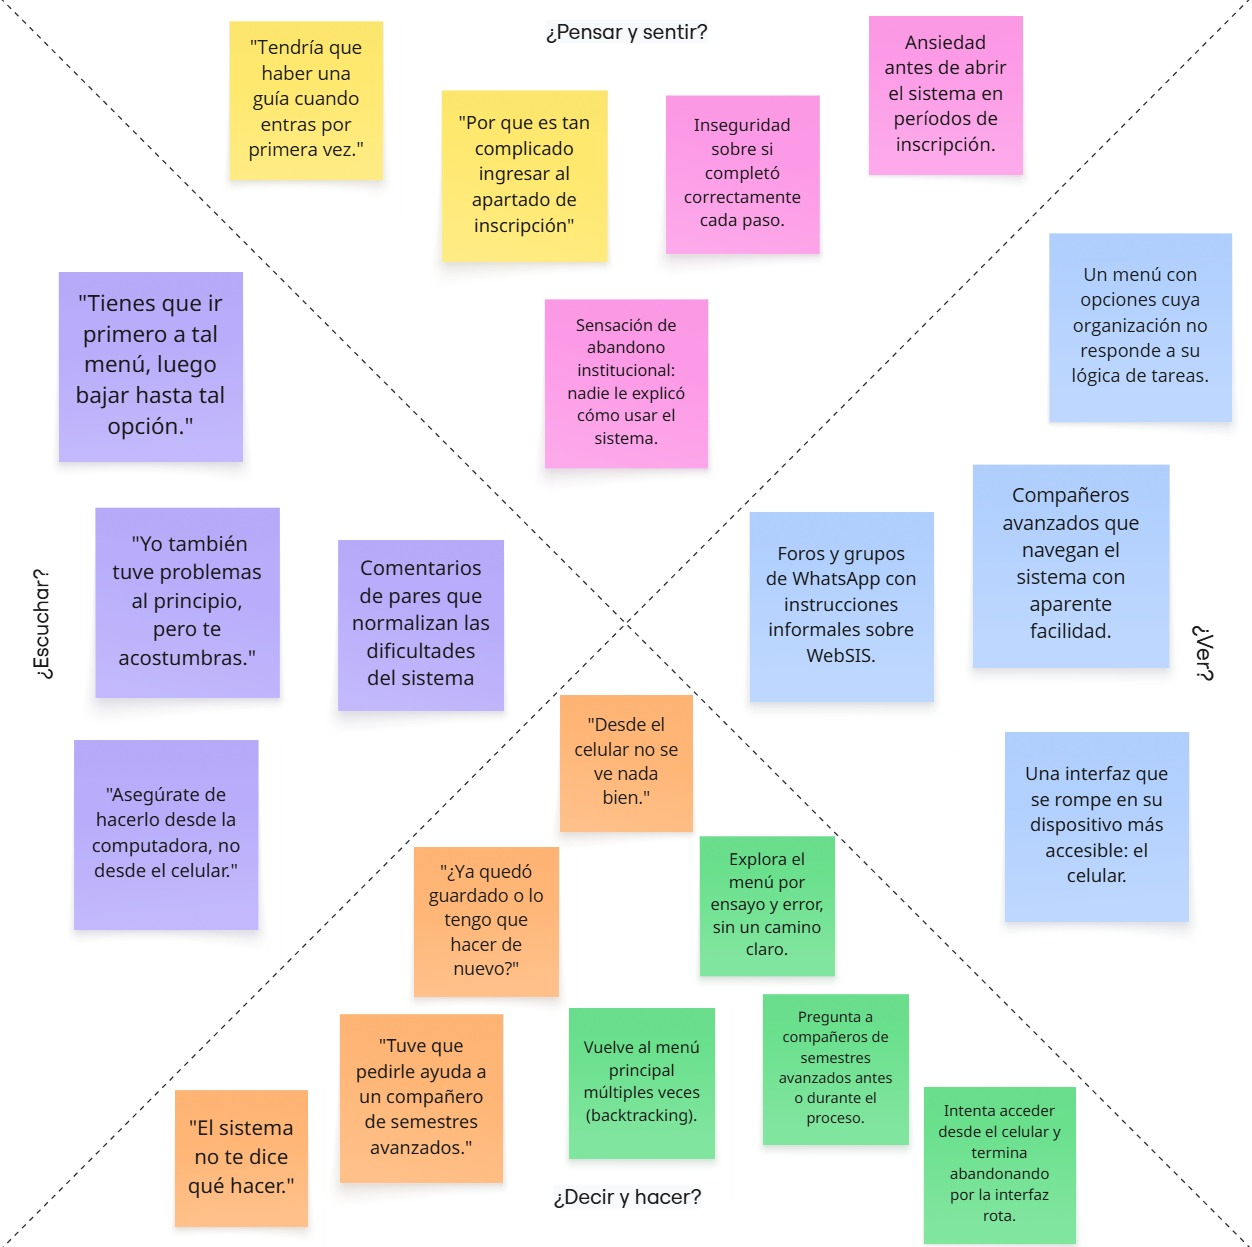
\includegraphics[width=0.85\textwidth]{images/nuevos.jpg}
    \caption{Mapa de empatía del estudiante ingresante}
    \label{fig:mapa-empatia-ingresante}
\end{figure}

La Figura~\ref{fig:beneficios-puntos-dolor-ingresante} muestra los beneficios esperados y los puntos de dolor identificados en la experiencia del estudiante ingresante con WebSIS.

\begin{figure}[H]
    \centering
    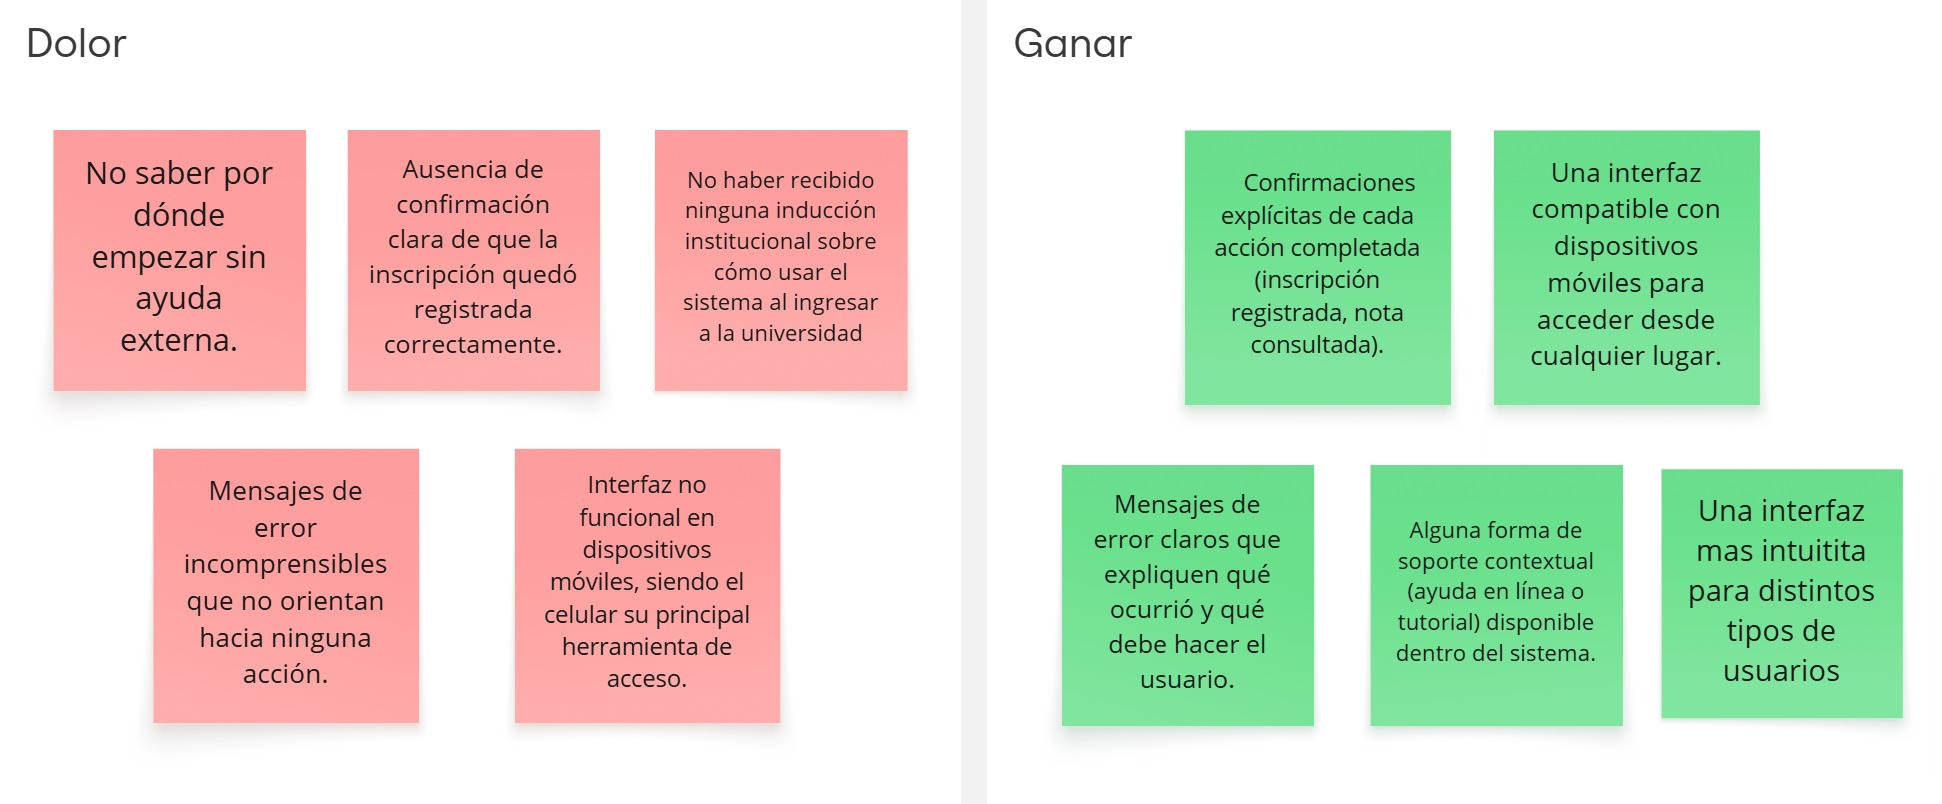
\includegraphics[width=0.95\textwidth]{images/nuevos1.jpg}
    \caption{Beneficios y puntos de dolor del estudiante ingresante}
    \label{fig:beneficios-puntos-dolor-ingresante}
\end{figure}

\subsubsection{Mapa de empatía - Perfil 2: Estudiante regular}

El mapa de empatía del estudiante regular sintetiza los hallazgos asociados a usuarios con mayor experiencia en WebSIS, elaborado en base a los usuarios Reynaldo, Adriana, Sebastián, Eduardo, Pablo, Junior, Diego y Mateo, considerando datos de encuesta, entrevistas E3, E4, E5, E7, E9, E10, E13 y E14, y la sesión de observación S2. Como se observa en la Figura~\ref{fig:mapa-empatia-avanzado}, este perfil evidencia estrategias de adaptación, búsqueda de eficiencia y desconfianza ante errores o caídas del sistema.

\begin{figure}[H]
    \centering
    \IfFileExists{images/avanzados.jpg}{%
        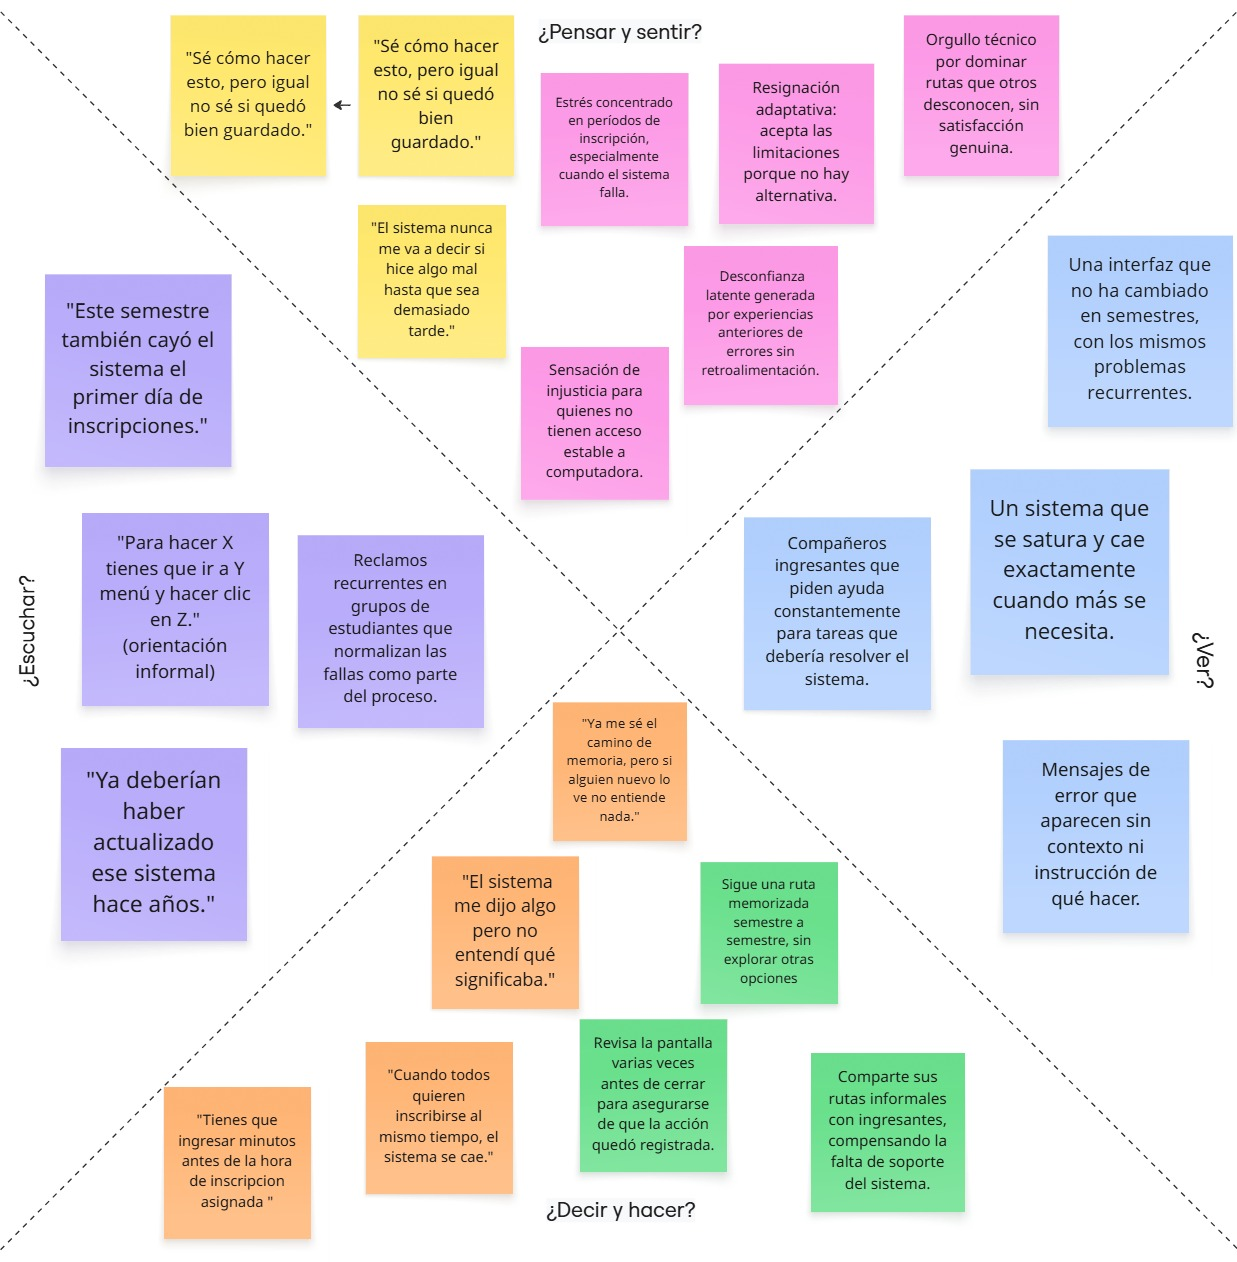
\includegraphics[width=0.85\textwidth]{images/avanzados.jpg}%
    }{%
        \fbox{\parbox{0.85\textwidth}{\centering Imagen pendiente: \texttt{images/avanzados.jpg}}}%
    }
    \caption{Mapa de empatía del estudiante regular}
    \label{fig:mapa-empatia-avanzado}
\end{figure}

La Figura~\ref{fig:beneficios-puntos-dolor-avanzado} presenta los beneficios esperados y los puntos de dolor identificados para el estudiante regular, destacando la necesidad de rapidez, confirmaciones claras y estabilidad durante períodos críticos.

\begin{figure}[H]
    \centering
    \IfFileExists{images/avanzados1.jpg}{%
        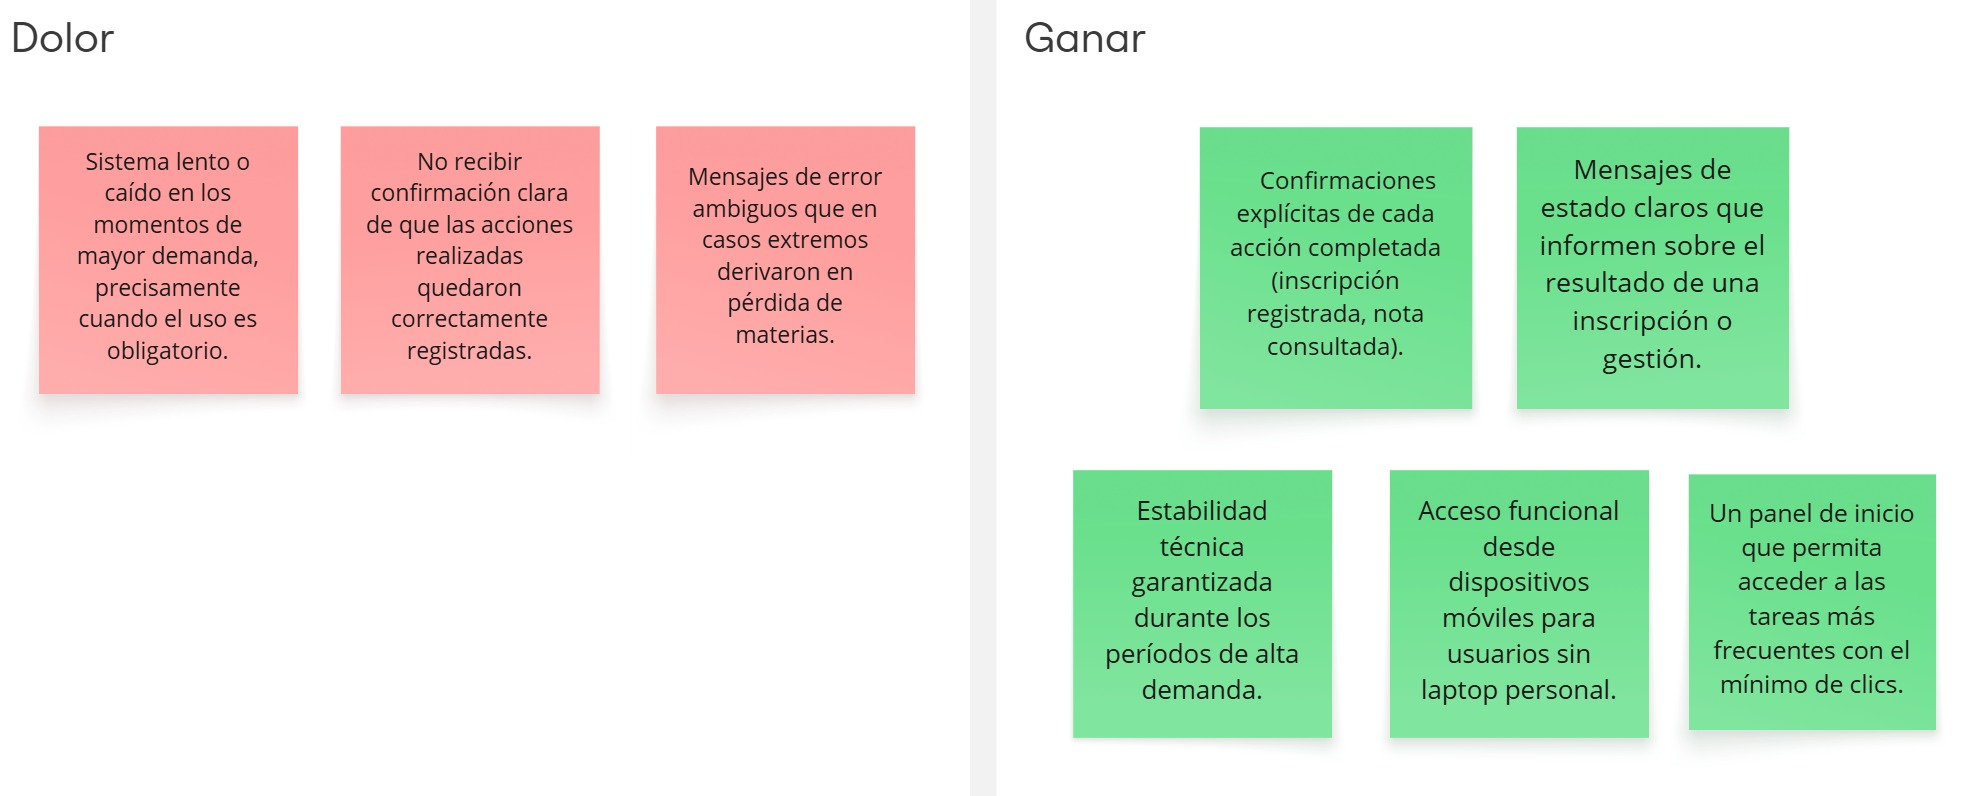
\includegraphics[width=0.95\textwidth]{images/avanzados1.jpg}%
    }{%
        \fbox{\parbox{0.95\textwidth}{\centering Imagen pendiente: \texttt{images/avanzados1.jpg}}}%
    }
    \caption{Beneficios y puntos de dolor del estudiante regular}
    \label{fig:beneficios-puntos-dolor-avanzado}
\end{figure}

\subsection{Escenarios de uso}

Los escenarios de uso narran, en forma de relato, cómo cada perfil enfrenta una tarea crítica dentro de su contexto real. Complementan a las personas porque sitúan las necesidades detectadas en una secuencia concreta de acciones, emociones y puntos de fricción, y sirven como referencia para evaluar si el rediseño responde a la experiencia esperada.

\subsubsection*{Escenario 1: Inscripción del estudiante ingresante}

\textbf{Persona:} Caleb, estudiante de primer semestre de Ingeniería Informática (Perfil 1). \\
\textbf{Contexto:} primer periodo de inscripción habilitado; accede desde su celular en casa, con conexión intermitente y bajo presión de plazos. \\
\textbf{Objetivo:} inscribirse a sus materias antes de que cierre la ventana habilitada.

Caleb ingresa a WebSIS por primera vez sin saber por dónde empezar. Necesita confirmar si su matrícula está pagada y si su cuenta está habilitada, pero no sabe dónde encontrar esa información. Al no recibir orientación, recurre a un compañero con mayor experiencia para que le indique la ruta. Cuando finalmente localiza el módulo de inscripción, duda si seleccionó los grupos correctos y si su inscripción quedó registrada, porque el sistema no le confirma el resultado. Termina la tarea con alivio, pero sin certeza de haberla completado bien.

\noindent\textbf{Necesidades involucradas:} N1 (guía en inscripción), N2 (confirmación de acciones), N4 (compatibilidad móvil), N6 (acceso rápido a tareas frecuentes), N8 (soporte contextual).

\subsubsection*{Escenario 2: Inscripción del estudiante regular}

\textbf{Persona:} Adriana, estudiante de séptimo semestre de Ingeniería Informática (Perfil 2). \\
\textbf{Contexto:} periodo de inscripción de alta demanda; accede desde su laptop, con experiencia acumulada pero desconfianza por errores previos. \\
\textbf{Objetivo:} completar la inscripción rápidamente y con la certeza de que las materias quedaron registradas.

Adriana conoce de memoria la ruta de inscripción, pero cada semestre debe reconstruirla porque la estructura no es evidente. Ingresa antes de la hora prevista por experiencias pasadas en que el sistema se atrasa o se satura. Selecciona sus materias con rapidez, pero revisa varias veces la pantalla porque teme que una acción no haya quedado guardada. La ausencia de una confirmación clara la obliga a verificar manualmente su estado de inscripción. Completa la tarea, pero con estrés y sin confiar plenamente en el resultado.

\noindent\textbf{Necesidades involucradas:} N2 (confirmación de acciones), N5 (navegación alineada al modelo mental), N6 (acceso rápido a tareas frecuentes), N7 (estabilidad técnica), N9 (autonomía académica).
